\documentclass[tikz,border=8pt]{standalone}
% Shared look for every TikZ diagram. Load with \input{../../tools/tikz-style.tex}
\usepackage[T1]{fontenc}
\usepackage{lmodern}
\renewcommand{\sfdefault}{lmr}  % diagrams use the same serif as the text
\usetikzlibrary{arrows.meta, positioning, shapes.geometric, calc, fit, backgrounds}
\definecolor{cblue}{HTML}{4C78A8}
\definecolor{corange}{HTML}{F58518}
\definecolor{cgreen}{HTML}{54A24B}
\definecolor{cred}{HTML}{E45756}
\definecolor{cpurple}{HTML}{B279A2}
\definecolor{cgrey}{HTML}{6B6B6B}
\tikzset{
  every picture/.style={font=\sffamily, line width=1.2pt},
  box/.style={draw=#1, fill=#1!12, rounded corners=4pt, align=center, inner sep=7pt, minimum height=1.1cm},
  box/.default=cgrey,
  arrow/.style={-{Stealth[length=3mm]}, draw=cgrey, line width=1.4pt},
  title/.style={font=\sffamily\bfseries\Large},
  note/.style={font=\sffamily\small, text=cgrey, align=center},
}
\AtBeginDocument{\hyphenpenalty=10000 \exhyphenpenalty=10000}

\begin{document}
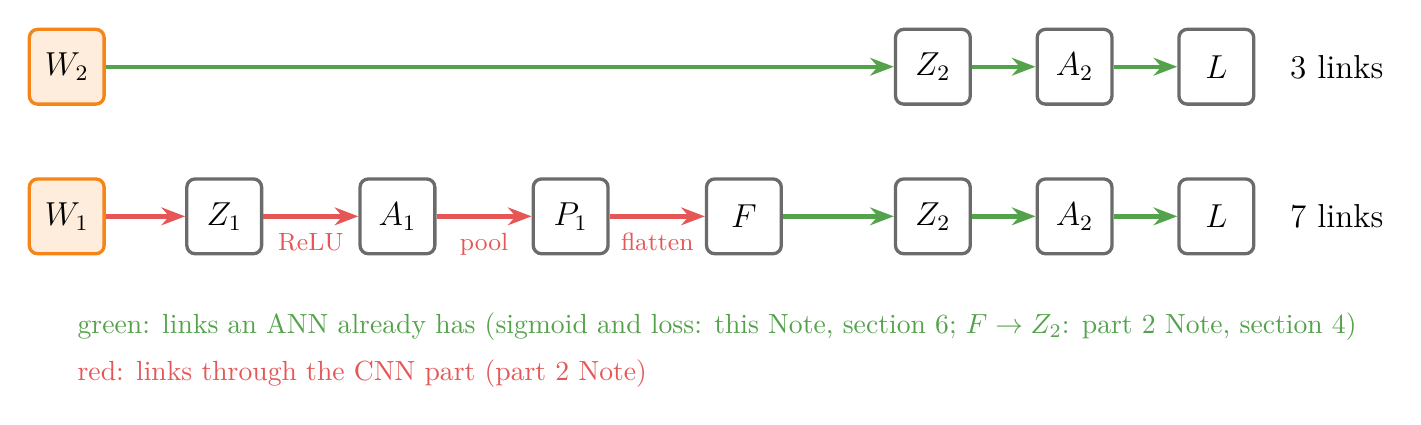
\begin{tikzpicture}[n/.style={draw=cgrey, fill=white, rounded corners=3pt, minimum size=0.95cm, font=\sffamily\large},
                    p/.style={n, draw=corange, fill=corange!15},
                    k/.style={-{Stealth[length=3mm]}, line width=1.6pt, draw=cgreen},
                    w/.style={-{Stealth[length=3mm]}, line width=1.6pt, draw=cred}]
  % W2 path
  \node[p] (w2) at (0,0) {$W_2$};
  \node[n] (z2a) at (11.0,0) {$Z_2$}; \node[n] (a2a) at (12.8,0) {$A_2$}; \node[n] (la) at (14.6,0) {$L$};
  \draw[k] (w2) -- (z2a); \draw[k] (z2a) -- (a2a); \draw[k] (a2a) -- (la);
  \node[anchor=west, font=\sffamily\large] at (15.4,0) {3 links};
  % W1 path
  \node[p] (w1) at (0,-1.9) {$W_1$};
  \foreach \t/\x [count=\i] in {Z_1/2.0, A_1/4.2, P_1/6.4, F/8.6, Z_2/11.0, A_2/12.8, L/14.6} \node[n] (q\i) at (\x,-1.9) {$\t$};
  \draw[w] (w1) -- (q1); \draw[w] (q1) -- node[below=2pt, font=\sffamily\small, text=cred] {ReLU} (q2);
  \draw[w] (q2) -- node[below=2pt, font=\sffamily\small, text=cred] {pool} (q3);
  \draw[w] (q3) -- node[below=2pt, font=\sffamily\small, text=cred] {flatten} (q4);
  \draw[k] (q4) -- (q5); \draw[k] (q5) -- (q6); \draw[k] (q6) -- (q7);
  \node[anchor=west, font=\sffamily\large] at (15.4,-1.9) {7 links};
  \node[font=\sffamily\normalsize, text=cgreen, anchor=west] at (0,-3.3) {green: links an ANN already has (sigmoid and loss: this Note, section 6; $F \to Z_2$: part 2 Note, section 4)};
  \node[font=\sffamily\normalsize, text=cred, anchor=west] at (0,-3.9) {red: links through the CNN part (part 2 Note)};
\end{tikzpicture}
\end{document}
